\documentclass[11pt]{article}
\usepackage[utf8]{inputenc}
\usepackage[T1]{fontenc}
\usepackage{natbib}
\usepackage{hyperref}
\usepackage{titling}
\usepackage[left=1in,right=1in,bottom=1in]{geometry}
\usepackage{setspace}
\usepackage{amsmath, amssymb}
\usepackage{float}
\usepackage{tikz}
\usepackage{booktabs}
\usetikzlibrary{positioning}

\setstretch{1.2}

\title{Deep Hedging with Non-Parametric Volatility Surfaces and Explicit Forecasting\\
\vspace{0.5em}
\large Learning from Market Data and Human Observable Information}
\author{Damanveer Singh Dhaliwal}
\date{\today}

\begin{document}
\maketitle

\section{Introduction}
Options hedging remains a critical aspect of quantitative finance, with traditional models such as the Black-Scholes delta hedging relying on strong assumptions. These assumptions, such as continuous rebalancing, constant volatility, no transaction costs, rarely hold in real markets. Given the crucial role of options hedging in financial risk management for banks, hedge funds and institutions, there is a pressing need for more robust and adaptive hedging strategies that can better capture market dynamics and uncertainties.

Recent advancements in machine learning, particularly deep reinforcement learning (DRL), have opened new avenues for developing sophisticated hedging strategies. Unlike traditional approaches that derive hedging ratios from closed form solutions under simplifying assumptions, DRL methods learn optimal hedging policies directly from data maximizing a reward function that reflects the hedger's objectives, such as minimizing risk or maximizing utility. This data-driven approach allows the DRL agent to navigate complex non-linearities and the transient nature of the financial markets without making any explicit assumptions of the underlying relationship.

Notably, \citet{buehler_deep_2018} showed the potential for deep hedging using RL and its potential to outperform traditional hedging strategies. \cite{francois2025enhancing} further demonstrate that deep hedging can significantly outperform classical methods, especially in markets characterized by frictions such as transaction costs and liquidity constraints. 

However, a notable limitation in the existing literature is the reliance on simulated market data generated from parametric stochastic volatility models such as the Heston or SABR (\cite{heston_closed-form_1993}). While these models capture certain parameters of the options markets, such as the volatility smiles and mean-reverting variances, they often fail to fully encapsulate the complexities and nuances of real-world market dynamics given their parametric nature. Activity such as regime shifts, liquidity crises, and market microstructures are very difficult to model accurately using these parametric frameworks.

To address these limitations, this paper proposes a novel approach to train deep hedging agents on real market data. Specifically, we use SPY options from 2011 to 2023, obtained from the WRDS OptionMetrics database. The intention is to allow the DRL agent to access the same information available to human traders: the full structure of the volatility surface across strikes and maturities. 

We employ a three-stage data pipeline to handle the high-dimensional and complex nature of the options data. First, we compress the 374-dimension volatility surface into a compact latent representation using an autoencoder. Second, an LSTM network forecasts the evolution of future volatility surfaces, providing the agent predictive information about the market. This is intended to replicate a human trader's implicit opinion of the future market conditions based on historical patterns. Finally, a reinforcement learning agent learns optimal hedging actions using these representations as state inputs. This three stage process allows us to investigate whether explicit forecasting improves performance and how the representation of the volatility surface impacts hedging effectiveness.

The rest of the paper is organized as follows. Section 2 reviews the relevant literature on deep hedging and place our work in context. Section 3 describes the data, model architecture and training methodology. Section 4 presents the empirical results and performance comparisons. Finally, Section 5 concludes with discussions on implications and future research directions.

\section{Literature Review}
\cite{buehler_deep_2018} presented the foundational work on deep hedging using reinforcement learning and established the theoretical and computational framework that launched the entire field. Their approach relies on using a Monte Carlo Policy gradient method to train a neural network on simulated price paths. The key results demonstrated that neural network based strategies can approximate optimal hedging solutions. 

There were two parallel strands of research that complemented this initial work. \cite{kolm_dynamic_2018} demonstrated that a deep reinforcement learning model agent learns to minimize variance in its hedge without explicit knowledge of volatility, the strike price or even the payoff function. It only requires the transaction costs and the price paths. This work highlighted the model-free nature of deep hedging and its ability to adapt to different market conditions.

During the same time, \cite{halperin_qlbs_2019} proposed the QLBS model, which combines reinforcement learning with the classical Black-Scholes-Merton framework. The QLBS model showed that option prices naturally emerge from the RL framework as the optimal value function, providing a bridge between traditional financial theory and modern machine learning approaches.

A significant methodological advancement was made by \cite{francois2025enhancing}, who introduced the use of the full implied volatility surface as part of the state representation for the RL agent. Their results indicated that incorporating the volatility surface led to substantial improvements in hedging performance, particularly in markets with transaction costs and liquidity constraints.

Other notable contributions to the deep hedging literature include \cite{carbonneau_deep_2020} who extends deep hedging to long-term derivatives like variable annuities and showed that non-quadratic penalties reduced downside risk in comparison to benchmarks. \cite{imaki_no-transaction_2023} introduced the no-transaction band network architecture that allows the agent to learn no-transaction regions, improving performance and training speed significantly. 

\cite{horvath_deep_2021} compare the performance of different hedging strategies under rough volatility models showing that deep hedging outperforms classical delta hedging in these more realistic settings. Finally, \cite{cao_deep_nodate} advanced the literature by introducing a distributional RL framework capable of optimizing mean-variance objectives. However, they also rely on simple low-dimensional state representations.

A critical gap in early deep hedging work is the reliance on simulated data. \cite{mikkila_empirical_2023} provided one of the first demonstration of training deep hedging agents on directly observed market pricing data. They find that a model trained on real market data outperforms one trained on simulated data when evaluated on real market conditions. However, their state representation is limited to a few summary statistics of the volatility surface rather than the full surface itself.

The literature reveals a clear trajectory where deep hedging provides a flexible and powerful framework for options hedging. However, existing work still relies heavily on simulated data and simplified state representations. This paper aims to address these gaps by training a deep hedging agent on real market data using the full volatility surface and incorporating explicit forecasting of future surfaces.

\section{Model Architecture}
\subsection{Black-Scholes-Merton Model}
The Black-Scholes(-Merton) model (\cite{black_pricing_1973}) is a foundational framework in financial mathematics for pricing European-style options. The model determines the price of an option based on the dynamics of the underlying asset's price and time. It assumes that the price of the asset follows a Geometric Brownian Motion with constant volatility and drift. It relies on 5 key variables: the current price of the underlying asset $S_t$, the strike price of the option $K$, the time to maturity $T-t$, the risk-free interest rate $r$, and the volatility of the underlying asset's returns $\sigma$.

The price of a European call option $C(S_t, t)$ under the Black-Scholes model is given by the formula:
\begin{equation*}
C(S_t, t) = S_t N(d_1) - K e^{-r(T-t)} N(d_2)
\end{equation*}
where:
\begin{equation*}
d_1 = \frac{\ln(S_t/K) + (r + \frac{\sigma^2}{2})(T-t)}{\sigma \sqrt{T-t}}, \quad d_2 = d_1 - \sigma \sqrt{T-t}
\end{equation*}
and $N(\cdot)$ is the cumulative distribution function of the standard normal distribution.

The model is a theoretical construct that provides closed-form solutions for option prices and subsequent hedging strategies. However, it relies on ideal market conditions that do not exist in practice, such as no transaction costs, continuous trading, and constant volatility. These limitations have led to the development of more sophisticated models and approaches, including the use of machine learning techniques like deep hedging.

\subsection{Reinforcement Learning}
Reinforcement Learning (RL) is a branch of machine learning where an agent learns to make sequential decisions through positive reinforcement to interact with an environment, with the goal of optimizing a reward or minimizing a penalty. The agent does this through trial and error, learning from the consequences of its actions over time. See \cite{sutton_reinforcement_2018} for a comprehensive introduction to RL.

In contrast to supervised learning, where the model learns from a labeled dataset, RL involves learning from the environment itself. Additionally, RL differs from unsupervised learning, which focuses on finding patterns in data without explicit feedback. In RL, the agent receives feedback in the form of rewards or penalties based on its actions, allowing it to learn optimal strategies over time.

In this paper, we will follow the notation of \cite{sutton_reinforcement_2018}. At each discrete time step $t$, the agent observes some representation of the environment's state $S_t \in \mathcal{S}$, where $\mathcal{S}$ is the set of all possible states, and selects an action $A_t \in \mathcal{A} (S_t)$, where $\mathcal{A} (S_t)$ is the set of actions available in state $S_t$. In the next time period, the agent receives a reward $R_{t+1} \in \mathcal{R} \subset \mathbb{R}$ based on its action and the environment transitions to a new state $S_{t+1}$ according to the environment's dynamics. The figure below diagrams the agent-environment interaction loop.

\begin{figure}[h]
    \centering
    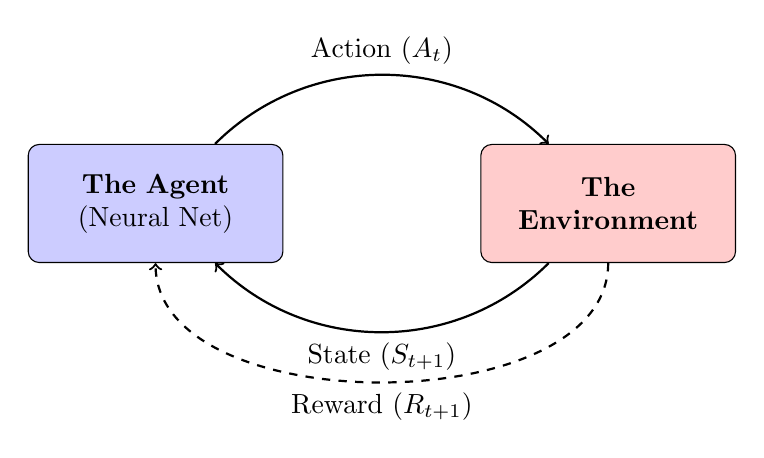
\begin{tikzpicture}[node distance=2.5cm, auto]
    % Nodes
    \node [rectangle, draw, fill=blue!20, text width=3cm, text centered, rounded corners, minimum height=1.5cm] (agent) {\textbf{The Agent} \\ (Neural Net)};
    \node [rectangle, draw, fill=red!20, text width=3cm, text centered, rounded corners, minimum height=1.5cm, right=of agent] (env) {\textbf{The \\ Environment}};

    % Arrows
    \draw [->, thick, bend left=45] (agent) to node [above] {Action ($A_t$)} (env);
    \draw [->, thick, bend left=45] (env) to node [below] {State ($S_{t+1}$)} (agent);
    \draw [->, dashed, thick] (env) to [out=270,in=270, looseness=0.9] node [below] {Reward ($R_{t+1}$)} (agent);
    \end{tikzpicture}
    \caption{RL Agent-Environment Interaction}
    \label{fig:rl_interaction}
\end{figure}

The agent's behavior is defined by a policy $\pi$, which maps states to actions. The goal of the agent is to learn an optimal policy $\pi^*$ that maximizes the expected cumulative reward over time, often discounted by a factor $\gamma \in [0,1)$ to prioritize immediate rewards over distant future rewards. The cumulative reward, or return, from time step $t$ is defined as:
\begin{equation*}
G_t = R_{t+1} + \gamma R_{t+2} + \gamma^2 R_{t+3} + \ldots + \gamma^T R_{T}
\end{equation*}
where $T$ is the terminal time step.

Reinforcement learning is particularly well-suited for problems like options hedging, where decisions must be made sequentially in a dynamic and uncertain environment. By learning directly from market data, RL agents can adapt to changing conditions and optimize hedging strategies without relying on rigid assumptions. 

Given that the financial objectives are clearly quantifiable, such as minimizing hedging error or maximizing risk-adjusted returns, RL provides a sophisticated framework for developing hedging strategies that can outperform traditional methods by adapting to market frictions like transaction costs. Additional explainable layers can be added to the architecture to ensure interpretability of the learned strategies.

\subsection{Proposed Architecture}
The proposed extension to the deep hedging framework introduced in \cite{francois2025enhancing} involves a three-stage architecture. First, we compress the high-dimensional volatility surface into a low-dimensional latent representation using an autoencoder. Second, we use an LSTM network to forecast future volatility surfaces based on historical data. Finally, we train a reinforcement learning agent to learn optimal hedging strategies using the latent representations and forecasts as state inputs. This architecture is designed to leverage the full information contained in the volatility surface while also incorporating predictive insights about future market conditions. 

The SPY options data used in this project consists of daily implied volatility surfaces spanning from 2011 to 2023 that were constructed from market prices downloaded from the Wharton Data Research Services (WRDS) \cite{OptionMetrics2025} database. 

A detailed description of each component's model and parameters has been presented below:
\subsubsection{Autoencoder for Volatility Surface Compression}
The volatility surface for SPY options is represented as a high-dimensional matrix, with dimensions corresponding to different strike prices and maturities. With 34 different delta and 11 maturities, the total number of dimensions balloons to $34 \times 11 = 374$. A representation of the data used is shown below:

\begin{figure}[H]
    \centering
    \includegraphics[width=1\textwidth]{../Output/Plots/ivs_surface.png}
    \caption{SPY Implied Volatility Surface}
    \label{fig:vol_surface}
\end{figure}
Using such a high-dimensional input directly in the RL agent is computationally intensive and may lead to overfitting. To address this, we employ an autoencoder, a type of neural network designed for unsupervised learning of efficient codings. The autoencoder consists of an encoder that compresses the input volatility surface into a low-dimensional latent space and a decoder that reconstructs the original surface from this latent representation.

The architecture of the autoencoder is as follows:
\begin{itemize}
    \item \textbf{Encoder:} The encoder consists of several convolutional layers followed by fully connected layers that reduce the dimensionality of the input volatility surface to a latent vector of size 32.
    \item \textbf{Decoder:} The decoder mirrors the encoder's architecture, using transposed convolutional layers to reconstruct the volatility surface from the latent vector.
    \item \textbf{Training:} The autoencoder is trained using mean squared error (MSE) loss between the original and reconstructed volatility surfaces. A ReLU activation function is used in the hidden layers, and 20\% dropout is applied to prevent overfitting. The Adam optimizer is used with a learning rate of 0.001, and training is performed for 200 epochs with a batch size of 64.
\end{itemize}
The figure below illustrates the architecture of the autoencoder used in this project (generated using Google's Nano Banana Pro AI Model):
\begin{figure}[H]
    \centering
    \includegraphics[width=1\textwidth]{../Output/Plots/autoencoder.png}
    \caption{Autoencoder Architecture for Volatility Surface Compression}
    \label{fig:autoencoder_architecture}
\end{figure}

The trained autoencoder achieves a reconstruction MSE of 0.1060 on the test set, indicating that it effectively captures the essential features of the volatility surface in the latent representation.

\subsubsection{LSTM for Prediction}
To provide the RL agent with predictive insights about future market conditions, we use a Long Short-Term Memory (LSTM) network to forecast the evolution of the volatility surface over time. The LSTM is well-suited for time series data due to its ability to capture long-term dependencies (\cite{fischer_deep_2017}).

During training, the LSTM takes as input 5 consecutive days of latent representations produced by the autoencoder with 32 dimensions each. The 5-day lookback window was chosen to capture short-term volatility dynamics and computational efficiency. Sensitivity analysis exploring alternative window lengths is left for future work. There are 2 stacked LSTM layers, the first processes the raw input sequence and the second processes the first LSTM's outputs. The ReLU activation function is used and a dropout of 30\% is applied to prevent overfitting. The Adam optimizer is used with a learning rate of 0.001, and training is performed for 200 epochs with a batch size of 32.

The LSTM is trained on the initial 80\% of the data to minimize the mean squared error, with the remaining 20\% reserved for test. The model's performance is evaluated using Mean Squared Error (MSE) between the predicted and actual latent representations of the volatility surface.

The performance of the LSTM model on the test set shows an MSE of 0.0281, indicating that the model effectively captures the temporal dynamics of the volatility surface but was unable to outperform a naive baseline that assumes the volatility surface remains constant over time.

\subsection{Reinforcement Learning Agent Design}
The final component of the architecture is the reinforcement learning agent, which is based on the agent used in \cite{francois2025enhancing}. The agent uses a RNN-FNN architecure to process the state inputs and learn optimal hedging strategies.

Once again, the training happens on the initial 80\% of the data, with the remaining 20\% reserved for test. The agent observes a state vector built from 5 base features: current price of the underlying asset, time remaining to expiration of the option being hedged, portfolio value, previous position and option type (call or put). Additionally, the agent observes current volatility features (either latent or the full surface) and the predicted volatility surface.

Each epoch runs 100 batches with normalized prices with $S_0 = 100$ and a strike price of $K = 100$. The normalization ensure consistent scaling across different time periods. The agent begins with the option premium received from selling the option that must be hedged. Subsequently, for each timestep $t$, the agent selects the number of shares to hold (as a hedge), calculate transaction costs based on the formula $cost = 0.01 \times price \times |\delta_{new} - \delta_{old}|$. The portfolio value is then calculated as $portfolio\_value = \delta \times (S_{t+1} - S_t) - cost$.

The payoff each timestep is calculated as what the hedger owes minus what they have in their portfolio. For a put option, this is shown below:
\begin{equation*}
{payoff}_t = \max(K - S_T, 0)
\end{equation*}
Similarly, for a call option, the payoff is:
\begin{equation*}
{payoff}_t = \max(S_T - K, 0)
\end{equation*}
The reward function is defined as the hedging error:
\begin{equation*}
    hedging\_error = payoff - portfolio\_value
\end{equation*}
The agent's objective is the minimize the MSE of the hedging error over the entire episode. The results from the agent's performance are presented in the next section.

\section{Empirical Results}
\subsection{Autoencoder Performance}
The performance of the autoencoder model is evaluated based on its ability to reconstruct the original volatility surface from the compressed latent representation. The reconstruction quality is measured using Mean Squared Error (MSE) between the original and reconstructed surfaces. A side-by-side comparison of the original and reconstructed volatility surfaces is shown below:
\begin{figure}[H]
    \centering
    \includegraphics[width=1\textwidth]{../Output/Plots/ae_results.png}
    \caption{Autoencoder Reconstruction Performance}
    \label{fig:autoencoder_performance}
\end{figure}
The autoencoder achieves a reconstruction MSE of 0.1060 on the test set, indicating that it effectively captures the essential features of the volatility surface in the latent representation. It can be observed that the reconstructed surface closely resembles the original, preserving key characteristics such as the volatility smile and term structure. However, some information loss is inevitable and can be seen that the reconstructed surface is smoother than the original especially in regions with high curvature.
\subsection{Predictor Performance}
The LSTM model's performance is evaluated based on its ability to forecast future volatility surfaces using the latent representation and the full volatility surface. The model's performance is measured using RMSE and compared against a naive baseline that assumes the volatility surface remains constant over time. A full time series plot of the predicted vs actual implied volatility for an at the money option is presented below:
\begin{figure}[H]
    \centering
    \includegraphics[width=1\textwidth]{../Output/Plots/lstm_full_timeseries.png}
    \caption{LSTM Prediction Performance on Full Volatility Surface}
    \label{fig:lstm_performance_full}
\end{figure}
This LSTM model was trained on the full volatility surface and achieved an RMSE of 0.0281 which was inferior to the naive baseline of 0.0150. The model struggled to isolate meaningful temporal patterns from the high-dimensional input data, leading to suboptimal predictions. We can observe this in the the figure above where the predicted values show a consistent lag.

In contrast, the LSTM model trained on the latent representation produced by the autoencoder achieved an RMSE of 1.2110, outperforming the naive baseline of 1.235. This highlights the advantage of using a compressed representation that captures the essential features of the volatility surface while filtering out noise. 

While the RMSE values are not directly comparable due to the differing feature spaces, the predictor using the latent representation demonstrates superior performance relative to its baseline, indicating that the autoencoder effectively distills relevant information for forecasting. In the next subsection, we will compare the hedging performance using both predictors to validate the economic value of these results.

\subsection{Hedging Agent Performance}
To evaluate the performance of the reinforcement learning hedging agent, we compare its hedging error against a classical delta hedging benchmark derived from the Black-Scholes-Merton model. The hedging error is calculated as the difference between the option payoff and the portfolio value at maturity, with lower values indicating better hedging performance. 

We also compare the performance of agents using different state representations and predictors. The RL-Hybrid agent uses a hybrid approach and combines the current compressed latent representation of the volatility surface with the predicted full volatility surface allowing the agent to leverage compact present information and rich predictive information. The results are summarized in the table below:
\begin{table}[H]
\caption{Comparative Hedging Performance (MSE \& RMSE) across 63-day Test Horizon}
\label{tab:hedging_results}
\resizebox{\linewidth}{!}{
\begin{tabular}{l|rrr|rrr}
\toprule
Strategy & Put MSE & Put RMSE & Put Imp (\%) & Call MSE & Call RMSE & Call Imp (\%) \\
\midrule
BS Delta (Baseline) & 9.0402 & 3.0067 & 0.0000 & 9.5158 & 3.0848 & 0.0000 \\
RL-Latent (No Pred) & 4.8462 & 2.2014 & 46.3932 & 7.6199 & 2.7604 & 19.9239 \\
RL-Latent (Pred) & 4.9841 & 2.2325 & 44.8673 & 11.3206 & 3.3646 & -18.9665 \\
RL-Full (No Pred) & 5.5338 & 2.3524 & 38.7873 & 9.8034 & 3.1310 & -3.0224 \\
RL-Full (Pred) & 7.7873 & 2.7906 & 13.8593 & 9.4257 & 3.0701 & 0.9465 \\
RL-Hybrid (Proposed) & 5.9724 & 2.4439 & 33.9350 & 10.3482 & 3.2169 & -8.7471 \\
\bottomrule
\end{tabular}}
\end{table}

These results clearly indicate that the RL framework consistently outperforms the Black-Scholes delta baseline for put options across all architectures, improving MSE by 33\% to 46\%. For call options, the results are mixed, with only the latent model without the predictions agent providing a substantial improvement over the baseline. 

We believe that the superior performance on put options is due to the volatility skew inherent in the equity index markets. The Black-Scholes model assumes constant volatility surface and thereby fails to capture any increase or decrease for any puts that command higher volatilities. For call options, the volatility surface is usually flatter and is closer to the Black-Scholes assumption of constant volatility, making the baseline more difficult to surpass. Given the difference in market dynamics for the training set (pre-pandemic) and the test set (post-pandemic), the RL agent received more room to learn effective hedging for puts.

It should also be noted that the inclusion of an explicit volatility forecast did not consistently improve performance over the latent agent other than the agent hedging call options that was trained on the full feature set. This suggests that the latent representation of the volatility surface likely encodes sufficient information for optimal hedging, and the explicit forecast introduces prediction noise that degrades the performance of the reinforcement learning agent. 

While the full feature set agent without prediction achieves reasonable performance on the puts, it shows signs of reduced generalization compared to the latent approach. Adding a predictor makes the dimensionality problem more severe and deteriorates performance.

\subsection{Robustness Checks with Synthetic Data}
To further validate the findings from our agent performance, we conduct robustness checks using synthetic data. Two sets of robustness checks were conducted:

The first one studied the performance of agents (that were trained on real data) on synthetic data that modeled four different market dynamics: a bull market, a bear market, and a crash and boom scenario. Synthetic data was generated using the geometric Brownian motion to model specific trends and risk levels associated with regimes that have been described before. 

To preserve realistic market structures, the corresponding implied volatility inputs were not generated synthetically. Instead, we employed a historical matching technique that assigned a real-world volatility surface sampled from the historical date with matching volatility characteristics to each synthetic regime. This approach allowed for controlled stress testing against hypothetical price movements while ensuring that the agent interacts with a valid complex volatility surface that contains all the information that a real one would. Results from this experiment are summarized in the table below:
\begin{table}[htbp]
\centering
\caption{Robustness Check: Hedging Performance across Synthetic Market Regimes}
\label{tab:synthetic_robustness}
\begin{tabular}{l|rr|r}
\toprule
Regime & RL MSE & BS MSE & Imp (\%) \\
\midrule
Bull Market & 2.3494 & 8.9816 & 73.8425 \\
Bear Market & 38.5404 & 10.6196 & -262.9172 \\
Crash & 199.1328 & 14.1400 & -1308.2939 \\
Boom & 4.9560 & 8.3824 & 40.8762 \\
\bottomrule
\end{tabular}
\end{table}


Given that the agents were trained on real market data, it is unsurprising that they perform well in the bull and boom regimes where market conditions are more stable and align with historical patterns. However, their performance degrades significantly in the bear and crash scenarios, where the market experiences sharp declines and heightened volatility. This suggests that while the agents have learned effective hedging strategies for typical market conditions, they struggle to adapt to extreme downturns that may not be well-represented in the training data.

To further investigate this, we conducted a second robustness check where the models were retrained entirely on synthetic data. Unlike the previous robustness check where constant volatility was assumed, this environment modeled volatility as a mean-reverting process with a negative 0.7 correlation to asset returns, capturing the leverage effect observed in real markets. Using this, we generated a 10-year synthetic dataset for the asset prices that was calibrated to match historical statistics. The synthetic implied volatility surfaces were constructed dynamically at each time step using the same approach as our real data, ensuring that the agent had access to realistic volatility information. The results from this experiment are summarized in the table below:
\begin{table}[H]
\centering
\caption{Pipeline Validation: End-to-End Performance on Synthetic Data}
\label{tab:synthetic_pipeline}
\begin{tabular}{lccccc}
\toprule
State Mode & Use Predictor & Is Put & Train Loss Final & Test Loss & State Dim \\
\midrule
latent & False & True & 3.4014 & 4.9388 & 37 \\
latent & False & False & 3.0406 & 6.2848 & 37 \\
latent & True & True & 1.4664 & 4.0171 & 69 \\
latent & True & False & 4.1015 & 5.6497 & 69 \\
full & False & True & 1.8134 & 4.7062 & 379 \\
full & False & False & 5.1245 & 5.7731 & 379 \\
full & True & True & 2.2938 & 8.3267 & 753 \\
full & True & False & 6.7536 & 6.8754 & 753 \\
hybrid & True & True & 1.9198 & 6.1425 & 411 \\
hybrid & True & False & 6.8405 & 6.7068 & 411 \\
\bottomrule
\end{tabular}
\end{table}


The results from the end-to-end synthetic pipeline provide strong empirical support for the proposed three-stage architecture. The reinforcement learning agent with the latent representation and access to a prediction achieved the lowest hedging error across all configurations, outperforming the static baseline. This confirms that in a controlled environment where volatility dynamics are mathematically coupled to the price, the latent predictor does extract and transmit valuable information that is forward-looking. 

The information that explicit forecasting did not provide sufficient information with real data but does with synthetic data supports the hypothesis that real-world volatility dynamics are more complex and results in academic research may not always translate directly to practice. It is likely that the LSTM model was learning some spurious patterns in the real data and thus was unable to provide useful information to the RL agent. This allows for future research directions to explore more sophisticated forecasting models.

Crucially, we can also observe that the reinforcement learning agent trained on the full dimensions clearly exhibited signs of overfitting, where it achieved a low training loss but the test loss was significantly higher, the worst among all the put strategies. This degradation validates our hypothesis that the curse of dimensionality thus prevents the reinforcement learning agent from making efficient decisions, and dimensionality reduction is a prerequisite for effective forecasting. By compressing the state-space, our architecture allows the agent to generalize better to unseen market conditions. 
\pagebreak
\section{Conclusion}
This paper addressed two key limitations in the existing literature of deep hedging:
1. The reliance on simulated data
2. The use of simplified state representations that discard information available to human traders
We solved for this by introducing a novel framework for deep hedging by training reinforcement learning agents directly on historical SPY options data from 2011 to 2023. The results of this experiment demonstrated that data-driven hedging strategies can substantially outperform classical delta hedging benchmarks. 

We propose a three-stage architecture comprising of:
1. An autoencoder compression
2. LSTM forecasting
3. Policy learning.
This design mirrors the decision-making process of a human trader who would have some forward-looking opinion based on historical patterns when constructing hedging strategies.

The empirical results revealed several important findings. First, the autoencoder successfully compressed the 374-dimensional volatility surface into a robust latent representation. Forecasting these latent dynamics proved significantly more accurate than attempting to predict the full surface directly, which failed to beat the naive baseline. 

Second, the deep hedging agents consistently outperformed the Black-Scholes Delta benchmark for put options, reducing the mean squared hedging error by approximately 46\% in the best-performing configuration. This confirms that the model can internalize volatility measures from the surface and correct for these to protect the underlying asset. However, for call options, the Black-Scholes model shows a baseline that was very difficult to surpass, probably because of the flatter volatility surface. However, our latent representation model was able to outperform it. 

Contrary to our initial hypothesis, the inclusion of explicit forecasting did not consistently improve hedging performance compared to the static latent agent in the real-world data. However, when we trained the model on synthetic data and evaluated its performance on synthetic data, the inclusion of explicit forecasting did provide valuable forward-looking information. This suggests that there is volatility in the real market dynamic that is unable to be captured by our prediction model. 

However, explicit forecasting did improve performance in the entirely synthetic data pipeline, confirming that in a controlled environment the explicit volatility-price modelling creates predictable patterns that the model is able to learn. In real markets, this relationship between volatility and prices changes often and is more complex, making it difficult for the LSTM to extract meaningful patterns.

We'd also like to acknowledge some of the limitations of the study. The experiments focused solely on at-the-money SPY options with a 63-day horizon, leaving open the question of how these results extend to different money levels, maturities, and underlying assets. The transaction cost model, while more realistic than frictionless assumptions, remains stylized compared to actual market microstructure. Additionally, the sequential training of the three pipeline stages may leave performance gains unrealized. 

These limitations allow us to envision some avenues for future research:
\begin{itemize}
    \item The framework can be extended to portfolio-level hedging, where agents manage books of options with correlated underlying assets rather than a single asset. This would test whether the learned representations capture cross-asset dependencies or not.
    \item Incorporating additional state variables such as macroeconomic indicators, or order flow data could further enhance predictive accuracy.
    \item Interpretability analysis of the learned policies would facilitate adoption by practitioners who require explainable decision making.
\end{itemize}


\pagebreak
\bibliographystyle{chicago}
\bibliography{references}

\end{document}